% =============================================================================
% Adaptive Green AI — arXiv preprint
% Generated from SOLUTION.md + patent inventive-core (M1..M6) and the
% frozen three-arm routing benchmark (run full-01).
%
% !! BEFORE POSTING TO arXiv / ANY PUBLIC SERVER !!
%   This describes an HPE patent disclosure. Public disclosure interacts with
%   patent rights (US 12-month grace vs. absolute-novelty jurisdictions).
%   Obtain HPE IP/legal clearance and confirm the provisional is filed FIRST.
%
% Build:  latexmk -pdf main.tex        (or)   pdflatex; bibtex; pdflatex x2
% arXiv accepts the standard `article` class + a .bbl file. See README.md.
% =============================================================================
\documentclass[10pt,twocolumn]{article}

\usepackage[margin=0.85in]{geometry}
\usepackage[utf8]{inputenc}
\usepackage[T1]{fontenc}
\usepackage{lmodern}
\usepackage{amsmath,amssymb}
\usepackage{booktabs}
\usepackage{graphicx}
\usepackage{xcolor}
\usepackage{tikz}
\usetikzlibrary{arrows.meta,positioning,fit,backgrounds}
\usepackage{hyperref}
\usepackage{cleveref}
\usepackage{siunitx}
\usepackage{listings}
\usepackage{authblk}
\usepackage{balance}

\hypersetup{colorlinks=true, linkcolor=blue!55!black, citecolor=green!45!black,
            urlcolor=blue!55!black}

\newcommand{\css}{\textsc{css}}
\newcommand{\gco}{\,\text{gCO}_2}
\newcommand{\gcokwh}{\,\text{gCO}_2/\text{kWh}}

\title{\textbf{Adaptive Green AI: Self-Tuning, Sustainability-Aware\\
Routing of LLM Requests with Per-Tenant Interpretable Policy Weights}}

\author[1]{Himanshu Tripathi}
\affil[1]{Hewlett Packard Enterprise \\ \texttt{himanshu.tripathi@hpe.com}}

\date{\today}

\begin{document}
\maketitle

\begin{abstract}
Large language model (LLM) inference is now a material and rapidly growing
source of data-center carbon emissions, yet production serving stacks route
requests almost exclusively on latency and cost. We present \emph{Adaptive
Green AI}, a carbon-aware LLM orchestration control plane that turns every
request into an explicit multi-objective routing decision over a pool of
heterogeneous model backends. The core is a \emph{Composite Sustainability
Score} (\css) that ranks candidate models along carbon, latency, accuracy, and
cost axes, with a carbon-dominant weighting derived from a live dual carbon
model (operational carbon via LLMCarbon-style accounting driven by real-time
grid carbon intensity, plus amortized embodied carbon). The \css{} weights are
\emph{interpretable}---four human-readable coefficients maintained
\emph{per tenant tier}---and \emph{self-tuning}: an online REINFORCE controller
updates them from every observed outcome, with no offline training step.
Two carbon-shifting primitives (temporal deferral to forecast low-carbon
windows and spatial reroute across grid zones) exploit the temporal and
spatial variability of grid carbon, and every decision is written to an
HMAC-signed, replayable ledger. We describe the system's six inventive
mechanisms and its implementation as a single FastAPI control plane over vLLM
backends, and we report a deliberately adversarial, fully frozen three-arm
benchmark (1{,}350 requests). The result is nuanced and stated without
overclaim: on a homogeneous small-model fleet an always-largest baseline is
Pareto-optimal, yet \css{} routing Pareto-dominates the carbon-blind heuristic
a competent engineer would write ($-5.6\%$ carbon at $+2.7$ quality points)
while remaining interpretable and auditable. We use the negative portion of
this result to characterize precisely when per-request carbon routing helps:
only when the model ladder contains a genuinely cheaper \emph{capable} rung.
Code, the benchmark harness, and the signed audit-log schema are released to
support reproducible carbon accounting.
\end{abstract}

\section{Introduction}
\label{sec:intro}

LLM inference has become a first-order data-center energy consumer: unlike
training, it runs continuously, scales with product adoption, and is dominated
by many small, latency-sensitive requests rather than a few large jobs. The
carbon cost of a request is the product of the energy it draws and the
\emph{carbon intensity} (CI) of the electricity serving it, and grid CI is far
from constant---it varies several-fold across regions and by roughly a factor
of two intraday within a single grid as the generation mix shifts between
renewables and fossil peakers~\cite{carbon-explorer,wait-awhile}. Production
serving stacks are blind to this: they select a backend to meet a latency or
cost target and treat the emitted carbon as an externality.

Existing model routers optimize a different objective. Learned and
blueprint routers such as RouteLLM~\cite{routellm} and the NVIDIA LLM
Router~\cite{nvidia-llm-router} choose a model to trade response quality
against dollar cost or latency, but carbon is out of scope and the learned
policy is typically opaque. Carbon accounting work such as
LLMCarbon~\cite{llmcarbon} models the operational and embodied footprint of a
model, but offline and after the fact. Carbon-aware scheduling
\cite{ecoserve,carbon-explorer,wait-awhile,carbon-aware-k8s} shifts batch and
training workloads in time and space toward cleaner energy, but has not been
folded into an interactive, per-request LLM router with service-level
constraints. No single system closes the loop \emph{grid $\to$ per-request
route $\to$ observed outcome $\to$ policy update} with carbon as the dominant,
acted-upon objective and an interpretable, per-tenant policy.

Adaptive Green AI is that closed loop. Every request is scored by a
carbon-dominant, SLA- and accuracy-gated Composite Sustainability Score
(\css) over a live candidate set; the carbon term is computed from a
dual (operational $+$ embodied) model driven by real-time grid CI; the \css{}
weights are four named coefficients maintained \emph{per tenant tier} and
updated online by a REINFORCE controller with no offline training phase; and
carbon-shifting primitives defer or reroute requests toward cleaner windows and
zones. Every decision---profile, weights, candidate breakdowns, carbon
decomposition, and observed outcome---is written to an HMAC-signed, replayable
ledger, so the routing rationale is auditable rather than asserted.

We also report an honest evaluation. On a controlled, fully frozen three-arm
benchmark over a homogeneous small-model fleet, an always-largest baseline is
Pareto-optimal on carbon \emph{and} quality, because on that fleet the lighter
rungs are not meaningfully cheaper per \emph{successful} answer. This is a
result, not a failure of the design: it isolates the precise precondition for
per-request carbon routing---a ladder with a genuinely cheaper capable rung---and
it lets us show what \css{} \emph{does} deliver even without that headroom, namely
a Pareto improvement over the carbon-blind heuristic an engineer would otherwise
write, at no loss of interpretability or auditability.

\medskip
\noindent\textbf{Contributions.} We claim:
\begin{enumerate}
  \item[\textbf{M1}] A per-request, carbon-dominant multi-objective routing
        score (\css) over heterogeneous LLM backends, gated by SLA and
        accuracy floors (\Cref{sec:m1}).
  \item[\textbf{M2}] A live dual carbon model combining operational carbon
        (LLMCarbon-style, driven by real-time grid intensity) and amortized
        embodied carbon, computed per candidate (\Cref{sec:m2}).
  \item[\textbf{M3}] Online reinforcement learning of the \css{} weights
        \emph{per tenant tier}, keeping the policy interpretable while
        self-tuning to observed outcomes (\Cref{sec:m3}).
  \item[\textbf{M4}] Carbon shifting via temporal deferral to forecast
        low-carbon windows and spatial reroute across grid zones
        (\Cref{sec:m4}).
  \item[\textbf{M5}] Semantic prompt profiling that selects the
        \emph{minimum-capability} model variant meeting the request's
        estimated requirements (\Cref{sec:m5}).
  \item[\textbf{M6}] An HMAC-signed, replayable carbon-decision ledger that
        makes every routing decision auditable and reproducible
        (\Cref{sec:m6}).
\end{enumerate}
The \emph{system} claim is the closed loop itself: grid and hardware carbon
$\to$ per-request \css{} routing $\to$ observed outcome $\to$ online per-tier
weight update $\to$ signed evidence. Beyond the mechanisms, a contribution of
this paper is the frozen benchmark harness (\Cref{sec:eval}) and its honest
negative-space finding on when such routing pays off.

\section{Related Work}
\label{sec:related}

\paragraph{LLM model routing.}
NVIDIA LLM Router~\cite{nvidia-llm-router} and learned routers such as
RouteLLM~\cite{routellm} select among models to trade quality against cost or
latency; RouteLLM trains a win-prediction router from human preference data to
send easy queries to a cheap model and hard ones to a strong model.
\emph{Delta:} these treat carbon as out of scope and optimize a cost- or
quality-only objective with an opaque learned policy. We make carbon a
first-class, dominant axis, keep the policy an interpretable four-weight vector
maintained per tenant tier, and gate it by explicit SLA and accuracy floors.

\paragraph{Carbon accounting for ML.}
LLMCarbon~\cite{llmcarbon} models the end-to-end operational and embodied
carbon of an LLM, and earlier work quantified ML emissions and argued for
efficiency as a first-class metric~\cite{mlco2,green-ai}. \emph{Delta:} those
estimates are computed offline for reporting; we drive an LLMCarbon-style
operational model with \emph{live} grid intensity per candidate at request time
and feed the result directly into the routing decision.

\paragraph{Carbon-aware scheduling and shifting.}
Temporal and spatial shifting of compute toward low-carbon windows and regions
has been studied for batch and training workloads and for datacenter design
\cite{ecoserve,carbon-explorer,wait-awhile,carbon-aware-k8s}; EcoServe in
particular targets carbon-aware AI inference systems~\cite{ecoserve}.
\emph{Delta:} we integrate deferral and reroute into an \emph{interactive},
per-request LLM router with tier-dependent delay tolerances, so shifting is one
option the same \css{} decision weighs against serving immediately.

\paragraph{Efficient LLM serving.}
vLLM~\cite{vllm} improves throughput and memory utilization via paged
attention, and sparse mixture-of-experts models~\cite{moe} raise parameter
efficiency. \emph{Delta:} this is orthogonal and complementary---we sit above
the serving engine and choose \emph{which} engine/model to invoke, folding MoE
all-to-all overhead into the carbon term rather than the serving loop.

\paragraph{Online policy learning for systems.}
Casting a systems control policy as an online-learned objective---bandit or
policy-gradient control of a scheduler or router---trades a hand-tuned
heuristic for one that adapts to observed reward. \emph{Delta:} we deliberately
restrict the policy class to a per-tier weight simplex updated by online
REINFORCE with an EMA baseline, so adaptivity does not cost interpretability:
the learned artifact is four named coefficients an operator can read.

\section{System Overview}
\label{sec:overview}

\begin{figure}[t]
  \centering
  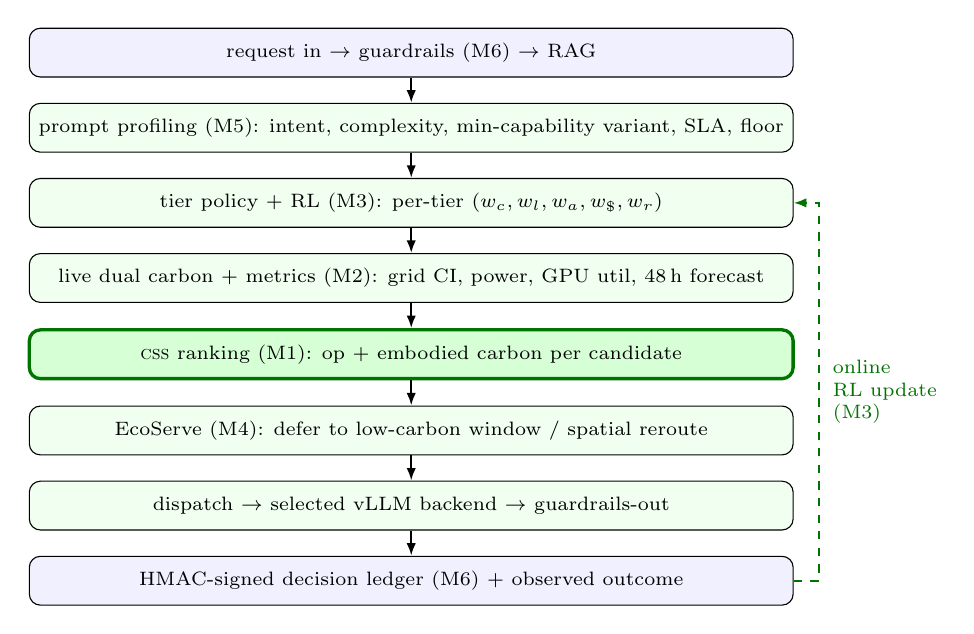
\begin{tikzpicture}[
      font=\scriptsize,
      node distance=3.2mm,
      stage/.style={draw, rounded corners, align=center, fill=green!6,
                    minimum width=0.80\columnwidth, minimum height=6.2mm,
                    inner sep=1pt},
      io/.style={stage, fill=blue!6},
      sel/.style={stage, fill=green!16, draw=green!45!black, very thick},
      arr/.style={-{Latex[length=1.6mm]}, thick}
    ]
    \node[io] (in) {request in $\to$ guardrails (M6) $\to$ RAG};
    \node[stage, below=of in] (prof) {prompt profiling (M5):
      intent, complexity, min-capability variant, SLA, floor};
    \node[stage, below=of prof] (pol) {tier policy $+$ RL (M3):
      per-tier $(w_c,w_l,w_a,w_{\$},w_r)$};
    \node[stage, below=of pol] (carb) {live dual carbon $+$ metrics (M2):
      grid CI, power, GPU util, 48\,h forecast};
    \node[sel, below=of carb] (css) {\css{} ranking (M1):
      op $+$ embodied carbon per candidate};
    \node[stage, below=of css] (eco) {EcoServe (M4):
      defer to low-carbon window / spatial reroute};
    \node[stage, below=of eco] (disp) {dispatch $\to$ selected vLLM backend
      $\to$ guardrails-out};
    \node[io, below=of disp] (aud) {HMAC-signed decision ledger (M6)
      $+$ observed outcome};

    \foreach \a/\b in {in/prof, prof/pol, pol/carb, carb/css, css/eco,
                       eco/disp, disp/aud}
      \draw[arr] (\a) -- (\b);

    % online feedback loop: outcome -> RL weight update
    \draw[arr, dashed, green!45!black]
      (aud.east) -- ++(3.2mm,0) |- (pol.east)
      node[pos=0.25, right, align=left]
        {\,online\\ \,RL update\\ \,(M3)};
  \end{tikzpicture}
  \caption{Adaptive Green AI control plane and the closed learning loop. Every
  request flows top-to-bottom through a fixed, auditable pipeline; the observed
  outcome (dashed) updates the per-tier \css{} weights online.}
  \label{fig:arch}
\end{figure}

Adaptive Green AI is a single control plane (FastAPI) in front of a pool of
heterogeneous vLLM backends. Every chat request follows a fixed, auditable
pipeline; each stage either enriches the request context or short-circuits with
a deterministic, logged substitute. \Cref{fig:arch} shows the loop and
\Cref{tab:pipeline} summarizes the routing-relevant stages.

\begin{table}[t]
  \centering
  \small
  \begin{tabular}{@{}p{0.30\columnwidth}p{0.60\columnwidth}@{}}
    \toprule
    \textbf{Stage} & \textbf{Output added to context} \\
    \midrule
    Prompt profiling (M5) & intent, complexity, min-capability variant, SLA, accuracy floor \\
    Tier policy + RL (M3) & per-tier $(w_c, w_l, w_a, w_{\$})$ \\
    Live carbon + metrics (M2) & grid CI, system power, GPU util, 48\,h forecast \\
    \css{} ranking (M1) & ranked candidates w/ op + embodied carbon \\
    EcoServe eval (M4) & deferral / reroute / low-carbon window \\
    Dispatch & selected vLLM endpoint \\
    Audit (M6) & HMAC-signed decision row \\
    RL update (M3) & new per-tier weights from observed outcome \\
    \bottomrule
  \end{tabular}
  \caption{Routing-relevant pipeline stages (the full pipeline has more stages
  for caching, multimodal dispatch, and persistence).}
  \label{tab:pipeline}
\end{table}

\section{Mechanisms}
\label{sec:mechanisms}

\subsection{M1: Composite Sustainability Score}
\label{sec:m1}

For each candidate $c$ in the live set, we min--max normalize each dimension
across the candidate set and form per-dimension scores in $[0,1]$ (higher is
better):
\begin{align}
s^{\text{carbon}}_c  &= 1 - \widehat{C}_c, \quad
s^{\text{lat}}_c      = 1 - \widehat{L}_c, \nonumber\\
s^{\text{acc}}_c     &= \widehat{A}_c, \quad
s^{\$}_c              = 1 - \widehat{\$}_c,
\end{align}
where $\widehat{\cdot}$ denotes min--max normalization over candidates (with
fixed anchors, e.g. accuracy over $[0.45, 1.0]$ and latency over
$[40\,\text{ms},\, L_{\max}{+}\text{MoE}{+}1.5\,\text{SLA}]$). The composite
score is the tier-weighted sum
\begin{equation}
\text{\css}_c = w_c\, s^{\text{carbon}}_c + w_l\, s^{\text{lat}}_c
              + w_a\, s^{\text{acc}}_c + w_{\$}\, s^{\$}_c
              + w_r\, s^{\text{region}}_c ,
\label{eq:css}
\end{equation}
with weights on the simplex ($\sum w = 1$, $w \ge w_{\min}$). The deployed
default weights are carbon-dominant---$w_c{=}0.60$ with
$(w_l,w_a,w_{\$},w_r){=}(0.12,0.16,0.08,0.04)$---so that carbon cannot be
outvoted by a single other axis, while latency and accuracy retain enough
influence to enforce their floors through the penalty terms below.
Interpretable adjustments then encode hard constraints as bounded
penalties/bonuses (\Cref{tab:adjust})---SLA overshoot, accuracy-floor
violation, semantic variant alignment, and a high-carbon-period penalty on
heavy variants. The highest adjusted \css{} wins; the top-$5$ candidates are
persisted for replay.

\begin{table}[t]
  \centering \small
  \begin{tabular}{@{}p{0.42\columnwidth}p{0.20\columnwidth}p{0.24\columnwidth}@{}}
    \toprule
    \textbf{Adjustment} & \textbf{Trigger} & \textbf{$\Delta$\css} \\
    \midrule
    SLA penalty & $L_c > \text{SLA}$ & $-\min(0.12{+}0.05o,\,0.25)$ \\
    Accuracy floor & $A_c < A_{\text{floor}}$ & $-0.18$ \\
    Semantic align & variant distance & $\pm0.14$ \\
    MoE complexity & moe $\wedge$ cplx${>}0.7$ & $+0.04$ \\
    High-carbon & CI${\ge}450$, heavy & $-0.05$ \\
    \bottomrule
  \end{tabular}
  \caption{Bounded, interpretable \css{} adjustments ($o$ = SLA overshoot ratio).}
  \label{tab:adjust}
\end{table}

\subsection{M2: Live Dual Carbon Model}
\label{sec:m2}

\paragraph{Operational carbon.} Following LLMCarbon-style
accounting~\cite{llmcarbon}, the per-request operational carbon of candidate
$c$ is
\begin{equation}
C^{\text{op}}_c = \frac{\text{TDP}_c \cdot t_c \cdot \text{PUE}_c}
                       {\text{HE}^{\text{eff}}_c \cdot 3.6\!\times\!10^{6}}
                  \cdot \text{CI} \cdot m_c,
\label{eq:op}
\end{equation}
where $t_c$ is estimated inference duration (s), $\text{HE}^{\text{eff}}$ folds
in MoE all-to-all overhead, $\text{CI}$ is \emph{live} grid carbon intensity
($\gcokwh$) from Electricity Maps, and $m_c$ a regional multiplier.

\paragraph{Embodied carbon.} Amortized per request over device lifetime:
\begin{equation}
C^{\text{emb}}_c = \frac{M_c \cdot 10^{3}}
                        {Y \cdot V \cdot \bar{t}} \cdot t_c,
\label{eq:emb}
\end{equation}
with manufacturing carbon $M_c$ (kg), lifetime $Y$ (yr), annual inference
volume $V$, and device-average duration $\bar t$. The routing carbon term is
$C_c = C^{\text{op}}_c + C^{\text{emb}}_c$; both components are stored per
candidate so the audit log proves the breakdown. \Cref{tab:params} lists the
deployed parameter values.

\begin{table}[t]
  \centering \small
  \begin{tabular}{@{}lll@{}}
    \toprule
    \textbf{Parameter} & \textbf{Symbol} & \textbf{Value} \\
    \midrule
    Power-usage effectiveness & PUE & $1.3$ \\
    Hardware efficiency & $\text{HE}$ & $0.68$--$0.72$ \\
    Per-variant board power & TDP & $95$--$310$\,W \\
    Manufacturing carbon & $M$ & $\approx 143$\,kg (A100-class) \\
    Device lifetime & $Y$ & $5$\,yr \\
    Annual inference volume & $V$ & $10^{5}$ \\
    Device utilization & --- & $0.35$ \\
    Device share (24\,GB slice) & --- & $0.255$ \\
    Grid intensity (live / bench) & CI & Electricity Maps / $475\gcokwh$ \\
    \bottomrule
  \end{tabular}
  \caption{Deployed dual-carbon parameters. At these settings embodied carbon
  is $1$--$3\%$ of the total, so the routing carbon term is
  operational-dominated.}
  \label{tab:params}
\end{table}

\subsection{M3: Online Per-Tenant Policy Learning}
\label{sec:m3}

Each tenant tier $\tau$ (standard / premium / esg / batch) carries its own
weight vector $w^{(\tau)}$. After each request we compute a bounded reward
\begin{equation}
R = \lambda_{\text{sla}} r_{\text{sla}} + \lambda_{\text{c}} r_{\text{c}}
  + \lambda_{\text{a}} r_{\text{a}} + \lambda_{\$} r_{\$} \in [0,1],
\end{equation}
and update the weights by online REINFORCE with an EMA baseline:
\begin{align}
\nabla_{w_i}\!\log \pi(a\!\mid\! s) &= s_i(a) - \mathbb{E}_\pi[s_i], \nonumber\\
w_i &\leftarrow w_i + \alpha_t\,(R - b)\,\nabla_{w_i}\!\log\pi, \\
\alpha_t = \tfrac{\alpha_0}{1+\sqrt{t}}, \quad
b &\leftarrow \beta b + (1-\beta)R , \nonumber
\end{align}
projected back onto the simplex with floor $w_{\min}$. Exploration uses sparse
Dirichlet perturbation ($\epsilon{=}0.15$) rather than discrete
$\epsilon$-greedy, so the policy stays a valid weight vector at all times.
Because the policy is four named weights, every update remains
\emph{human-interpretable} and per-tenant---an operator can read off why a tier
routes the way it does. The deployed tiers already differ in a legible way:
the \texttt{esg} tier carries $w_c{=}0.70$ and the \texttt{premium} tier
$w_c{=}0.45$ (with correspondingly higher latency/accuracy weight), so the same
mechanism expresses distinct sustainability postures without a separate model.
This interpretability-preserving, per-tenant online update is the design's core
differentiator from opaque learned routers.

\subsection{M4: Carbon Shifting (Defer + Reroute)}
\label{sec:m4}

When CI is high ($\ge 450\gcokwh$), the request tolerates delay
(tier-dependent deferral budget), the target supports batching, and the 48\,h
forecast contains a window at least $15\%$ lower in CI within budget, the
request is enqueued and dispatched in that window
(\texttt{find\_low\_carbon\_window}). Independently, if multi-region grid
signals expose a zone with materially lower CI, the request is flagged for
spatial reroute. Because these primitives move a fixed unit of work to cleaner
energy rather than choosing a cheaper model, their carbon benefit does
\emph{not} depend on the model ladder having a cheaper capable rung---which,
as \Cref{sec:eval} shows, is exactly the regime where per-model routing has
little to exploit.

\subsection{M5: Minimum-Capability Prompt Profiling}
\label{sec:m5}

A sentence-transformer encodes the prompt against prototype banks (route,
priority, intent) and STEM keyword sets to estimate intent, a complexity score
in $[0,1]$, and the \emph{minimum} model variant expected to meet the request's
accuracy floor and SLA. This biases the candidate set toward the greenest
feasible model before \css{} scoring. A hashed-vector fallback preserves the
contract when the encoder is unavailable.

\subsection{M6: Signed, Replayable Decision Ledger}
\label{sec:m6}

Every decision is appended as one JSON line carrying the full semantic profile,
policy coefficients (with RL version/exploration flags), the top-5 candidate
\css{} breakdowns, the selected candidate's carbon decomposition, eco-actions,
retrieval/grounding traces, guardrail traces, live grid and system metrics,
observed latency/accuracy, and token/GPU carbon---signed with HMAC-SHA256 over
the canonical body. Any post-hoc tampering invalidates the line, and any
decision can be replayed from its row. This ledger is also the single source of
truth for all operational dashboards, eliminating metrics drift.

\section{Implementation}
\label{sec:impl}

The control plane is a FastAPI service ($\approx$\,15{,}000 lines of Python
across the routing, learning, and accounting modules, exposing roughly $50$
HTTP/WebSocket endpoints) orchestrating routing
(\texttt{routing\_policies.py}), online RL (\texttt{rl\_controller.py}), hybrid
RAG (\texttt{advanced\_rag.py}), carbon and system monitoring
(\texttt{monitoring\_layer.py} plus a host-metrics sidecar), a versioned model
registry with MoE placement (\texttt{model\_zoo.py}), a carbon-aware deferred
queue (\texttt{deferred\_queue.py}), programmable guardrails
(\texttt{nemo\_guardrails.py}), and the signed audit writer; a React\,19
frontend renders the live grid, policy, queue, and metrics state. Backends are
vLLM containers. The registered zoo spans a $0.345$B model
(DialoGPT-medium), a $1.1$B dense model (TinyLlama-1.1B), $1.5$B dense
instruct/STEM specialists (Qwen2.5-1.5B and Qwen2.5-Coder-1.5B), a $7.6$B coder
(Qwen2.5-Coder-7B-AWQ), a $30$B sparse MoE (Qwen3-30B-A3B), CPU fallbacks
(Llama-2-7B, DialoGPT), and pluggable NVIDIA NIM endpoints for vision (VLM) and
diffusion image generation. Every external dependency has a deterministic
fallback (encoder $\to$ hashed embeddings; grid API $\to$ cached $+$ default CI;
\texttt{nvidia-smi} $\to$ estimated utilization; cross-encoder $\to$ heuristic;
vLLM $\to$ rule-based extractive), so the pipeline degrades gracefully. The
evaluation below runs on an NVIDIA vGPU slice (\texttt{H100L-2-24C}, a $24$\,GB
slice of a $\sim$$94$\,GB board) at PUE $1.3$.

\section{Evaluation}
\label{sec:eval}

We evaluate with a deliberately adversarial harness whose design goal is to
make it \emph{hard} for the router to look good: a single frozen router, one
prompt set, and every learning and caching mechanism disabled so that the
measurement reflects the routing \emph{policy} and not a drifting environment.
We report the result without overclaim, including where the router does not win.

\subsection{Research Questions}
\begin{itemize}
  \item \textbf{RQ1.} How much carbon does \css{} routing save versus an
        always-largest baseline and versus a carbon-blind static heuristic, at
        comparable task quality?
  \item \textbf{RQ2.} What is the mechanism behind the RQ1 result---i.e., what
        property of the model ladder determines whether per-request routing can
        save carbon?
  \item \textbf{RQ3.} Do the learned per-tier policies remain interpretable and
        differ by tier?
  \item \textbf{RQ4.} What carbon-saving headroom does carbon shifting (M4)
        offer independent of the ladder?
\end{itemize}

\subsection{Setup}
Three arms share one prompt set of $150$ prompts across seven categories (code,
extraction, factual, general, math, reasoning, summarization), each replayed
$3\times$ ($1{,}350$ requests total). \textbf{always-full} pins every prompt to
the largest available backend (a $1.5$B instruct model). \textbf{static-heuristic}
is a carbon-blind client-side rule (prompt length $+$ keywords $\to$
small/medium/full)---the heuristic a competent engineer writes in an
afternoon, and the real bar to clear. \textbf{css} is the full router with no
pin. To make the arms comparable, the harness freezes every confounder: the
semantic cache, RL exploration and weight updates, and the quality/latency
estimator are all disabled; grid CI is pinned at $475\gcokwh$ so it scales all
arms identically; and the MoE reconciler and LLM guardrail classifiers are off.
Requests carry no shared conversation context and zero deferral tolerance, and
each arm uses a distinct tenant id so a missed freeze surfaces as contamination
rather than passing silently. \textbf{Carbon} is ex-post: spec TDP $\times$
\emph{measured} wall-clock, billed to the model that actually served, summed
over every inference leg (a retry bills both). \textbf{Quality} is a
lower-bound objective-checker pass rate (numeric-with-tolerance, substring,
regex, executed-code asserts; no LLM judge), with the same checker on every
arm. Power is modeled, not measured---the vGPU slice reports
\texttt{power.draw = [N/A]}, so TDP is an upper bound on real draw.

\subsection{Results}

\begin{table}[t]
  \centering \small
  \begin{tabular}{@{}lrrrr@{}}
    \toprule
    \textbf{Arm} & \textbf{$\gco$/req} & \textbf{vs full} &
    \textbf{Quality} & \textbf{p50} \\
    \midrule
    always-full      & $0.0187$ & ---       & $79.3\%$ & $1234$\,ms \\
    static-heuristic & $0.0218$ & $+16.6\%$  & $62.0\%$ & $1614$\,ms \\
    \css             & $0.0206$ & $+10.0\%$  & $64.7\%$ & $1364$\,ms \\
    \bottomrule
  \end{tabular}
  \caption{Headline results (run \texttt{full-01}, $1{,}350$ requests, grid CI
  pinned). Carbon and quality are both ex-post and measured with the same
  procedure across arms.}
  \label{tab:headline}
\end{table}

\Cref{tab:headline} is the headline, and it is nuanced.
\emph{(i)~Against always-full (RQ1):} on this fleet the always-largest baseline
is Pareto-optimal---it has both the lowest carbon and the highest quality---and
\css{} spends $10\%$ \emph{more} carbon at $14.7$ fewer quality points. We do
not claim a win here.
\emph{(ii)~Against the static heuristic:} \css{} Pareto-dominates the realistic
carbon-blind baseline, using $5.6\%$ less carbon ($0.0206$ vs $0.0218$) at
$+2.7$ quality points and with no pin violations (the heuristic incurred $102$).
The interpretable, carbon-aware policy is strictly better than the rule an
engineer would otherwise ship, which is the comparison that matters once
``just use the big one'' is off the table for cost or capacity reasons.

\subsection{Why always-full wins (RQ2)}
The mechanism is the fleet, not the router. The largest routinely-available
backend here is only a $1.5$B instruct model, and the lighter rungs
(TinyLlama-1.1B and below) are not meaningfully cheaper \emph{per successful
answer}: they emit substantially more output tokens (mean $\sim$$121$ vs $75$
for the full model) and score far lower on math ($25.3\%$ vs $76.0\%$) and
reasoning ($40.0\%$ vs $53.3\%$), so the compute they save is given back as
longer generations and lost quality. The $30$B MoE and $7$B coder that would
constitute genuinely cheaper-per-capability rungs are registered in the zoo but
were not live backends in this fleet. The finding generalizes as a precondition:
\emph{per-request carbon routing saves carbon only when the ladder contains a
rung that is both cheaper and capable enough for a non-trivial fraction of
traffic.} On a homogeneous small-model fleet that rung does not exist, and the
honest routing move is to serve the strongest model---which the carbon-dominant
\css{}, via its accuracy-floor penalty, already does for the hard categories
(summarization $95.6\%$, above always-full's $84.4\%$).

\subsection{Interpretability of learned policies (RQ3)}
Because the policy is a four-weight simplex per tier, the learned artifact is
directly readable. The shipped tiers already encode distinct, legible
postures---$w_c$ ranges from $0.45$ (\texttt{premium}) to $0.70$
(\texttt{esg})---and online updates keep the vector on the simplex, so an
operator can always state why a tier routed as it did. This is the property
opaque learned routers cannot offer, and it holds regardless of the ladder
result above.

\subsection{Carbon shifting (RQ4)}
Temporal deferral and spatial reroute (M4) move a fixed unit of work toward
cleaner energy, so their benefit is bounded by grid-CI variability
(several-fold spatial, $\sim$$2\times$ intraday~\cite{carbon-explorer,wait-awhile})
rather than by the model ladder. This is orthogonal to RQ1--RQ2 and is
\emph{not} exercised by the frozen benchmark (deferral tolerance is pinned to
zero so requests cannot leave the run). We therefore report M4 as a
design-level capability, not a measured saving, and flag an end-to-end
grid-trace evaluation of it as the primary open item.

\subsection{Threats to Validity}
Power is modeled from TDP, an upper bound, because the vGPU exposes no
per-request draw; the reported carbon is therefore a conservative ceiling, not
a meter reading. Quality is a lower bound from objective checkers, so absolute
levels are pessimistic though the cross-arm comparison is fair. Grid CI is
pinned, which is the correct control for comparing routing policies but removes
exactly the variability M4 exploits---so this benchmark cannot credit M4. The
result is a single-fleet finding; a fleet with a genuinely cheaper capable rung
(e.g. a live $30$B MoE beside the small dense models) could move the RQ1
comparison, and confirming that is future work. Embodied carbon depends on
\texttt{device\_utilization} ($0.35$), the one free parameter; at this setting
it is $1$--$3\%$ of the total, so the headline is operational-dominated.

\section{Discussion and Limitations}
\label{sec:discussion}
The central lesson is that per-request model routing only converts to carbon
savings when the model ladder has headroom---a rung that is both cheaper and
capable for real traffic. When it does not, as on our small-model fleet, the
carbon-optimal choice collapses to ``serve the strongest model,'' and the
value of a carbon-aware router shifts from \emph{which model} to \emph{when and
where} to run it (M4) and to \emph{governance}: an interpretable, per-tenant,
signed policy that provably did the right thing. Our contribution is honest on
both halves: we show \css{} beating the realistic carbon-blind heuristic and we
show the ceiling that the fleet imposes. Limitations follow directly---the
result depends on the grid-CI signal quality for M4, on the presence of a
cheaper capable rung for M1, and on the expressive limits of a four-weight
linear policy, which we accept deliberately in exchange for interpretability.

\section{Conclusion}
\label{sec:conclusion}
Adaptive Green AI makes carbon a first-class, acted-upon objective across
routing, SLA gating, MoE go/no-go, temporal deferral, spatial reroute, and the
RL reward, with an interpretable per-tenant policy and an HMAC-signed decision
ledger as evidence. Our frozen benchmark shows the router Pareto-dominating the
carbon-blind heuristic while remaining auditable, and---just as
usefully---characterizes exactly when per-request routing pays off: only with a
genuinely cheaper capable rung in the ladder. The mechanisms that do not depend
on that precondition (carbon shifting and interpretable governance) are where
the largest remaining carbon headroom lies.

\section*{Availability and Reproducibility}
The control plane, the frozen three-arm benchmark harness, and the signed
audit-log schema are released to enable reproducible carbon accounting; every
reported number in \Cref{tab:headline} is regenerable from the harness
(run \texttt{full-01}). A repository/DOI link will be added after HPE IP/legal
clearance.

\section*{Ethics and Disclosure}
This work describes an HPE patent disclosure; public release follows HPE policy
and provisional filing. It involves no human subjects. All carbon figures are
model-based and reported with their assumptions (\Cref{tab:params}, RQ2--Threats):
power is modeled from TDP rather than metered, quality is a lower bound, and
grid intensity is pinned for the comparison.

\balance
\bibliographystyle{plain}
\bibliography{references}

\end{document}
